\clearpage\begingroup\SourceLeaf{64}\NoSourceHead\HistoricalFoot{}{8\textsuperscript{*}}
\begin{center}
{\Large NACHLASS.}\\[1.3em]
{\large [BERECHNUNG MAGNETISCHER KRÄFTE.]}\par\medskip
\rule{.86\textwidth}{.35pt}\\
{\small [Aus Handbuch 15, Ba, Opuscula varii argumenti.\quad Volumen primum.\quad Brunovici 1800.]}\\
\rule{.86\textwidth}{.35pt}\\[.8em]
[1.]
\end{center}
\noindent{\small [S. 174]}
\begin{center}\textbf{Zierliche Construction für die magnetische Ablenkung.}\end{center}
\begin{center}
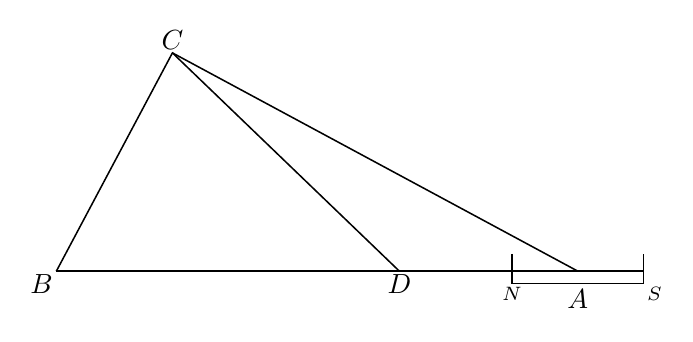
\begin{tikzpicture}[x=.022cm,y=.022cm,line width=.55pt]
\coordinate (B) at (0,0);\coordinate (C) at (67,126);
\coordinate (D) at (198,0);\coordinate (A) at (301,0);
\draw (B)--(C)--(A);\draw (C)--(D);\draw (B)--(339,0);
\draw (263,10)--(263,-7)--(339,-7)--(339,10);
\node[below left,inner sep=1pt] at (B) {$B$};
\node[above,inner sep=1pt] at (C) {$C$};
\node[below,inner sep=1pt] at (D) {$D$};
\node[below,inner sep=2pt] at (301,-7) {$A$};
\node[below,inner sep=1pt] at (263,-7) {$\scriptstyle N$};
\node[below right,inner sep=1pt] at (339,-7) {$\scriptstyle S$};
\end{tikzpicture}
\end{center}
\noindent\hspace*{\parindent}\begin{tabular}{@{}ll@{}}
\(A\)&Centrum eines Magnets\\
\(SN\)&Richtung seiner Axe\\
\(AB\)&deren Fortsetzung\\
\(C\)&ein Element freien Magnetismus\\
\(CB\)&senkrecht auf \(AC\)\\
\multicolumn{2}{@{}l@{}}{\(AD=\frac{1}{3}AB\)}
\end{tabular}\par
Dann wird, wenn der Magnetismus in \(C\) südlicher ist, solcher in der
Richtung \(CD\) angezogen; ist er nördlicher, in der entgegengesetzten abgestossen
mit einer Intensität
\[
=\frac{DC}{AD\mathpunct{.}AC^3}\times M,
\]
\noindent wo \(M\) das statische Moment des freien Magnetismus des Magnets in \(A\) ist.
\clearpage\endgroup
